
\tikzset{vecteur/.style={->,thick,color=black,smooth}}

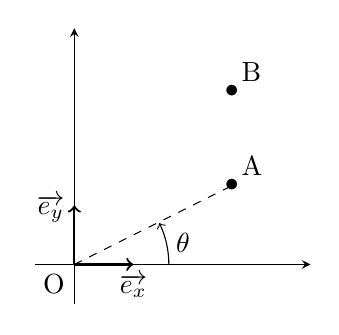
\begin{tikzpicture}[
	base/.style={>=latex},
	axis/.style={->,>=stealth},
	M/.style={rectangle,draw,fill=lightgray,minimum size=0.5cm,thin},
	m/.style={rectangle,draw=black,fill=lightgray,minimum size=0.3cm,thin},
	plane/.style={draw=black,fill=blue!10},
	string/.style={draw=red, thick},
	pulley/.style={thick},
	]
	
	\coordinate (O) at (0, 0) ;
	\draw (O) node[below left] {O};
	
	
	\draw [axis] (-0.5,0)--(3,0); 
	\draw [axis]  (0,-0.5) --(0,3);   
	\draw (0.75,0) node[below]  {$\overrightarrow{{e}_{x}}$} ++(-0.75,1) 
	node[below left]  {$\overrightarrow{{e}_{y}}$};
	
	\coordinate (B) at (2,2.2);
	\draw (B) node[above right] {B};
	\draw (B) node{$\bullet$} ;
	
	\coordinate (A) at (2,1);
	\draw (A) node[above right] {A};
	\draw (A) node{$\bullet$} ;
	\draw[->] (1.2,0) arc (0:26:1.2) ;
	\draw (13:1.2) node[right] {$\theta$}; 
	\draw[dashed] (O) -- (A);
	\draw[vecteur] (O)-- ++(0.75,0);
	\draw[vecteur] (O)-- ++(0,0.75);

\end{tikzpicture}
